\documentclass[a4paper, 12pt]{article}%тип документа

%отступы
\usepackage[left=2cm,right=2cm,top=2cm,bottom=3cm,bindingoffset=0cm]{geometry}

%Русский язык
\usepackage[T2A]{fontenc} %кодировка
\usepackage[utf8]{inputenc} %кодировка исходного кода
\usepackage[english,russian]{babel} %локализация и переносы

%Вставка картинок
\usepackage{wrapfig}
\usepackage{graphicx}
\graphicspath{{pictures/}}
\DeclareGraphicsExtensions{.pdf,.png,.jpg}

%оглавление
\usepackage{titlesec}
\titlespacing{\chapter}{0pt}{-30pt}{12pt}
\titlespacing{\section}{\parindent}{5mm}{5mm}
\titlespacing{\subsection}{\parindent}{5mm}{5mm}
\usepackage{setspace}

%Графики
\usepackage{multirow}
\usepackage{pgfplots}
\pgfplotsset{compat=1.9}

%Математика
\usepackage{amsmath, amsfonts, amssymb, amsthm, mathtools}

%Стиль страницы
\usepackage{fancyhdr}
\pagestyle{fancy}

\begin{document}

\begin{titlepage}

\begin{center}
%\vspace*{1cm}
\large\textbf{Московский Физико-Технический Институт}\\
\large\textbf{(национальный исследовательский университет)}
\vfill
\line(1,0){430}\\[3mm]
\huge\textbf{Лабораторная работа №4.5.2}\\
\large\textbf{Интерференция лазерного излучения}\\
\line(1,0){430}\\[1mm]
\vfill
\large Баканова К.В., Б01-003\\
%\vspace*{1cm}
\large март 2022 г.\\
\end{center}

\end{titlepage}
\textbf{Цель работы}: исследование зависимости видности интерференционной картины излучения гелий-неонового лазера и определение длины когерентности излучения.


\textbf{В работе используются}: He-Ne-лазер, интерферометр Майкельсона с подвижным зеркалом, фотодиод с усилителем, осциллограф, поляроид, линейка.
\section*{Теория}
\subsection*{Гелий-неоновый лазер}
Лазер представляет собой интерферометр Фабри-Перо -- газовую трубку с двумя параллельными зеркалами по обе стороны. В лазере длиной $L$ для излучения вдоль оси для резонансных частот выполняется
\begin{equation}
\nu_m = \dfrac{mc}{2L}.
\end{equation}
В этом случае генерируется несколько волн -- \textit{мод} -- межмодовое расстояние для которых
\begin{equation}
\Delta \nu = \nu_{m+1} - \nu_m = \dfrac{c}{2L}.
\end{equation}
\subsection*{Видность}
Видность интерфереционной картины -- параметр, определяемый формулой
\begin{equation}
\gamma = \dfrac{I_{max} - I_{min}}{I_{max} + I_{min}},
\end{equation}
где $I_{max}$, $I_{min}$ -- максимальная и минимальная интенсивности света интерфереционной картины вблизи выбранной точки. Разобьём его на произведение функций параметров установки
$$
\gamma = \gamma_1 \gamma_2 \gamma_3.
$$
Здесь $\gamma_1$ отвечает за соотношение интенсивности интерферирующих волн:
\begin{equation}
\gamma_1 = \dfrac{2\sqrt{\delta}}{1+\delta},
\end{equation}
где $\delta = \frac{B_m^2}{A_m^2}$, $A_m$ и $B_m$ -- амплитуды волн. Параметр $\delta$ определяется устройством разделения волн.\\
Функция $\gamma_2$ возникает вследствие немонохроматичности волн.
\begin{equation}
	\gamma_2 = \bigg | \frac{1}{n}\frac{\sin\frac{\pi l}{2L}n}{\sin\frac{\pi l}{2L}} \bigg |,
\end{equation}

\subsection*{Установка}
\begin{figure}[h]
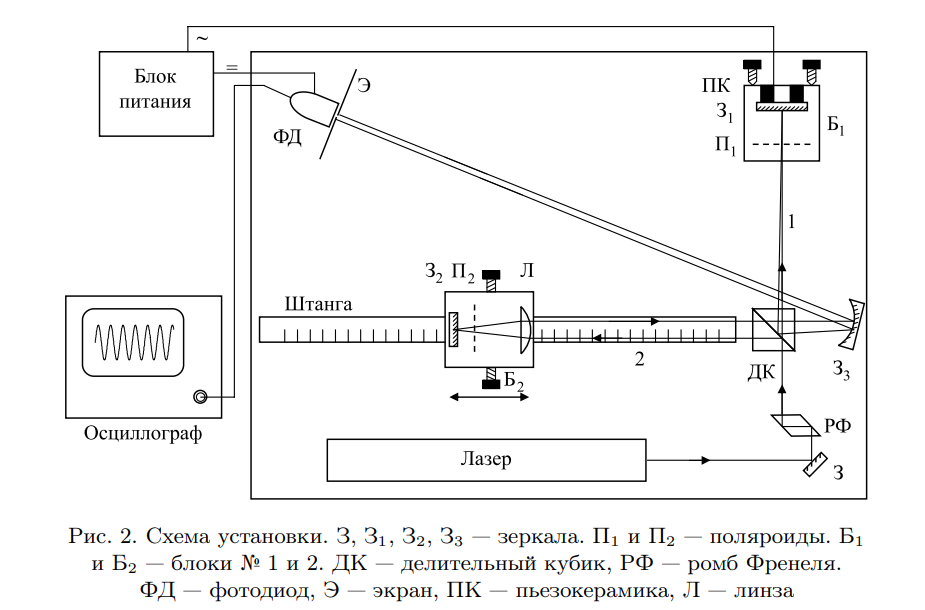
\includegraphics[scale=0.75]{2.png}
\centering
\caption{Схема установки.}
\end{figure}
Источником света служит гелий-неоновый лазер (средняя длина волны $\lambda_0$ = 632,8 нм). Пучок лазерного излучения отражается от зеркала З и проходит призму полного внутреннего отражения РФ (ромб Френеля), которая превращает линейную поляризацию излучения в круговую. Если в установке используется лазер, излучающий неполяризованный свет, то ромб Френеля не нужен, но он и не мешает выполнению работы. Далее лазерное излучение делится диагональной плоскостью делительного кубика ДК на два пучка.

Пучок 1 проходит поляроид П1, отражается под небольшим углом от зеркала З1, снова проходит поляроид П1 и, частично отражаясь от диагональной плоскости делительного кубика, выходит из интерферометра, попадает на зеркало З3 и далее на фотодиод ФД. Зеркало З1 наклеено на пьезокерамику ПК, которая может осуществлять малые колебания зеркала вдоль направления распространения падающего пучка. Поляроид и зеркало с пьезокерамикой собраны в единый блок Б1, который крепится к вертикально стоящей плите. В блоке Б1 имеются юстировочные винты, которые позволяют регулировать угол наклона зеркала З1. В установке предусмотрена возможность вращения поляроида П1. Угол поворота отсчитывается по шкале, нанесённой на оправу поляроида.

Пучок 2 проходит линзу Л, поляроид П2, отражается от зеркала З2, снова проходит поляроид П2, линзу Л и делительный кубик, выходит из интерферометра, попадает на зеркало З3 и далее на фотодиод ФД. Таким образом, от зеркала З3 под небольшим углом друг к другу идут на фотодиод два пучка, прошедшие разные плечи интерферометра. Между ними происходит интерференция и образуются интерференционные полосы. Линза Л, поляроид П2 и зеркало З2 собраны в единый блок Б2. Зеркало З2 установлено в фокальной плоскости линзы Л. Это сделано для того, чтобы падающий и выходящий из блока Б2 пучки всегда были
параллельны друг другу. Блок Б2 может перемещаться вдоль пучка 2 по штанге, жёстко связанной с плитой интерферометра. Длина штанги 90 см. В установке предусмотрена возможность небольшого поперечного перемещения блока Б2, что позволяет регулировать расстояние между падающим и выходящим из блока пучками. При измерениях блок Б2 крепится к штанге при помощи двух винтов. Вдоль штанги нанесены деления через один сантиметр. При перемещении блока Б2 вдоль штанги на величину $x_1$ геометрическая разность хода между пучками 1 и 2 изменяется на величину $l = 2x_1$.

\subsection*{Измерение видности}
Типичная осциллограмма сигнала фотодиода приведена на рис. 2. По осциллограмме можно найти следующие величины: фоновую засветку (линия 0 — перекрыты оба пучка 1 и 2); интенсивность света каждого из пучков (линии 1 или 2 — перекрыт пучок 2 или 1); максимума и минимума интенсивности интерференционной
картины (открыты оба пучка). При этом параметр $\delta$, необходимый для расчёта $\gamma_1$ в формуле (4), определяется данным

\begin{wrapfigure}{l}{0.4\textwidth}
\begin{center}
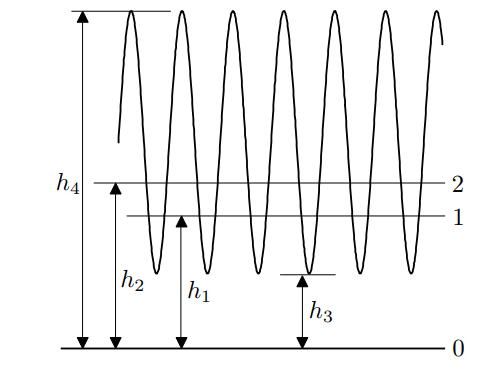
\includegraphics[width = 0.4\textwidth]{3.png}
\vspace{-40pt}
\end{center}
\caption{Осциллограмма сигналов фотодиода.}
\end{wrapfigure}

соотношением
\begin{equation}
\delta = \dfrac{h_1}{h_2},
\end{equation}
Видность интерференционной картины рассчитывается по формуле: 
\begin{equation}
\gamma = \dfrac{h_4 - h_3}{h_4 + h_3},
\end{equation}
Здесь 0 -- уровень при отсутствии лучей, 1 и 2 -- при закрытии одного из них.\\ 
При условии одинаковой поляризации лучей ($\beta = 0$), т.е. когда ($\gamma_3 = 1$)
\begin{equation}
\gamma_2 = \dfrac{\gamma}{\gamma_1}.
\end{equation}
\\ Если же разность хода отсутствует ($l = 0$), или же ($\gamma_2 = 1$) то для известного угла $\beta$
\begin{equation}
\gamma_3 = \dfrac{\gamma}{\gamma_1}.
\end{equation}
\section*{Ход работы}
Пронаблюдаем интерференционную картину на экране. Поставим дополнительный поляроид между лазером и ПФ, вращая его, наблюдаем, что поляризация линейная. Перенесём поляроид и поставим его на пути луча, выходящего из ПФ. Наблюдаем, что теперь у луча круговая поляризация. Установим минимальную чёткость интерфереционной картину вращением $\text{П}_1$. Внесём дополнительный поляроид на пути луча, идущего на экран, -- интерфереционная картина вновь возникает из-за поляризованности света, так как после прохождения второго поляроида два луча будут иметь одну поляризацию, задаваемую поляроидом.\\
Исследуем зависимость видности интерфереционной картина от угла $\alpha$ между плоскостями поляризации интерферирущих лучей. В нашем случае $\alpha$ -- угол поворота поляроида $\text{П}_1$. Результаты измерений представлены в Таблице 1. При подсчётах были использованы формулы (8), (5), (9) и (11). Погрешность измерения угла приборная $\sigma_\alpha = 1^\circ$, погрешность измерения всех $h$ -- половина цены деления $\sigma_{h_i} = 0.1 \text{ дел}$. Для $\gamma_3$ погрешность вычисляется по формуле 
$$
\sigma_{\gamma_3} = \sqrt{\sum\limits_{i=1}^4\left(\dfrac{\partial \gamma_3}{\partial h_i}\right)^2 \sigma^2_{h_i}}.
$$


\begin{table}[h]
\begin{tabular}{|c|c|c|c|c|c|c|}
\hline
$\beta$ & $h_1$, дел & $h_2$, дел & $h_3$, дел & $h_4$, дел & $\gamma_3$ & $\sigma_{\gamma_3}$ \\ \hline
0        & 0.2        & 0.4        & 1.4        & 1.7        & 0.1       & 0.07      \\ \hline
30       & 0.2        & 0.4        & 1.0        & 2.2        & 0.4       & 0.07      \\ \hline
60       & 0.2        & 0.4        & 0.6        & 2.3        & 0.6       & 0.07      \\ \hline
90       & 0.2        & 0.4        & 0.5        & 2.9        & 0.7       & 0.07      \\ \hline
120      & 0.2        & 0.4        & 0.5        & 1.9        & 0.6       & 0.07      \\ \hline
165      & 0.2        & 0.4        & 1.0        & 1.2        & 0.1       & 0.07      \\ \hline
\end{tabular}
\centering
\caption{Результаты измерений для $\gamma_3 = \gamma_3(\beta)$.}
\end{table}

\begin{figure}[h]
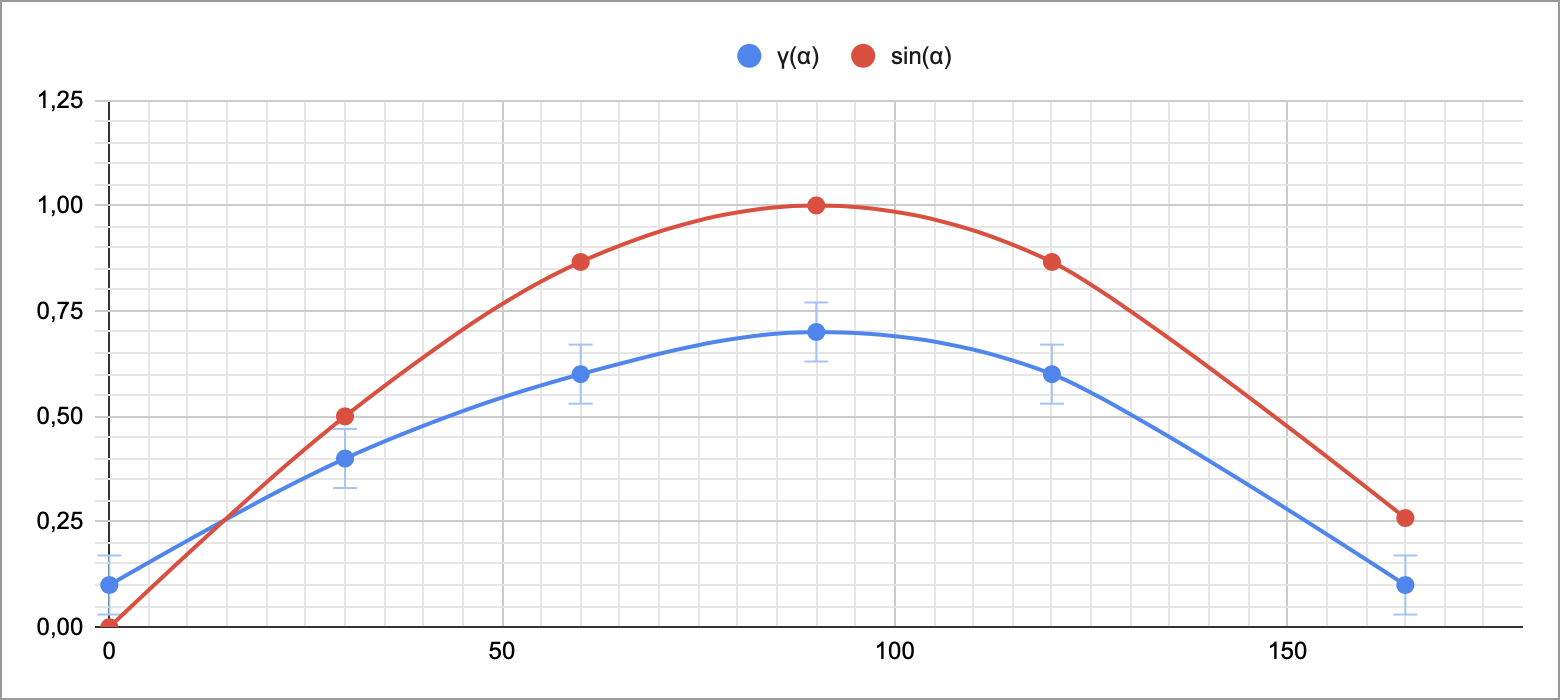
\includegraphics[scale=0.6]{4.png}
\centering
\caption{Сравнение $\gamma_3(\beta)$ и $\cos(\beta)$.}
\end{figure}
\newpage
Теперь исследуем зависимость видимости интерфереционной картины от разности хода между лучами. Для этого будем перемещать блок $\text{Б}_2$ вдоль направления распространения луча, координата блока $x$ будет определять разность хода. Значения измерений представлены в Таблице 2, а так же на графике (Рис. 4).\\
На графике явно видны два максимума -- на $x_1 = 16\pm 2 \text{ см}$ и на $x_2 = 80 \pm 2 \text{ см}$. Тогда $L = \frac{1}{2}(x_2 - x_1) = 32.0 \pm 1.4 \text{ см}$. Отсюда из формулы (2)
$$
\Delta \nu = \dfrac{c}{2L} = (47 \pm 2) \cdot 10^7 \text{ Гц}.
$$
Погрешность считается из соотношения $\varepsilon_{\Delta\nu} = \varepsilon_{L}$. Полуширина кривой из графика
$$
l_{1/2} \approx 12 \pm 2 \text{ см},
$$
откуда по формуле:
$$
\Delta \nu_{\text{полн}} = 0.6\dfrac{c}{l_{1/2}} = (145 \pm 38) \cdot 10^7 \text{ Гц}.
$$
Погрешность считается аналогично $\Delta \nu$. Тогда по формуле число мод:
$$
N = 1 + 1.2\dfrac{L}{l_{1/2}} = 4.2 \pm 0.6, 
$$
погрешность рассчитана по формуле:
$$
\sigma_N = \sqrt{\left( \dfrac{\partial N}{\partial \Delta \L} \right)^2 \sigma^2_{\Delta \L} + \left( \dfrac{\partial N}{\partial \Delta \l_{1/2}} \right)^2 \sigma^2_{\Delta \l_{1/2}}}
$$
с округлением до целых.
\begin{figure}[h]
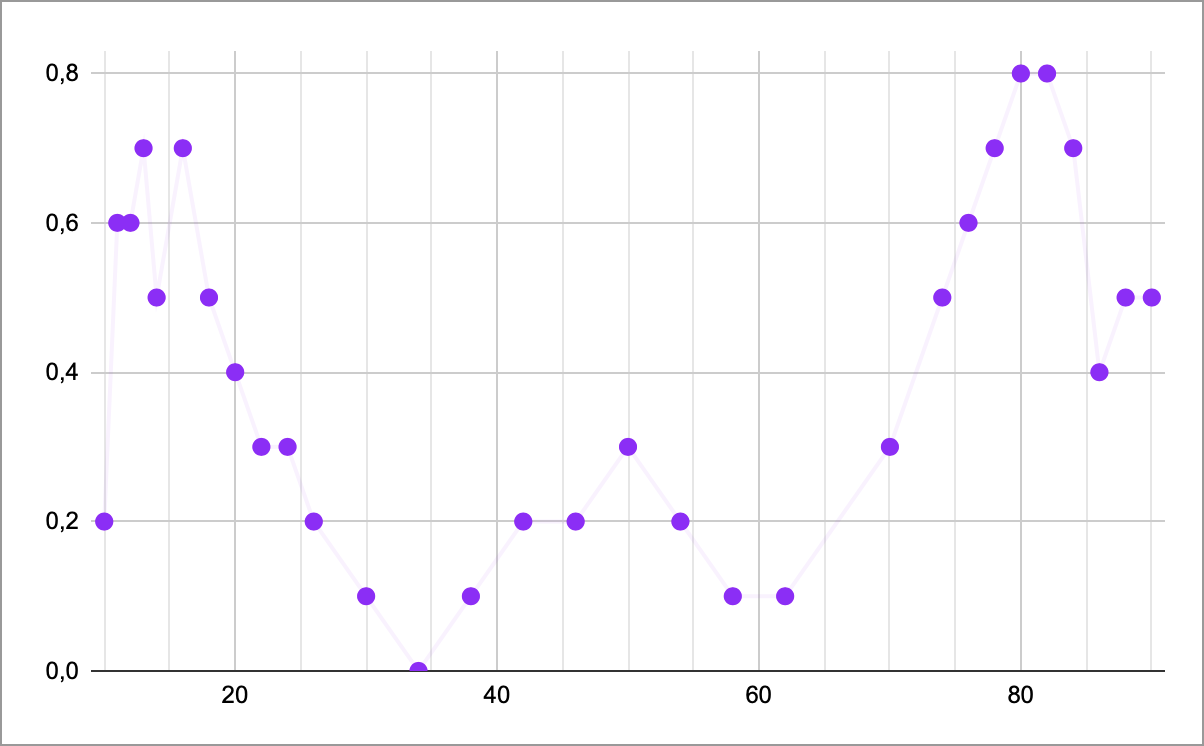
\includegraphics[scale=0.6]{5.png}
\centering
\caption{Зависимость $\gamma_2 = \gamma_2(x)$.}
\end{figure}
\begin{table}[H]
\begin{tabular}{|c|c|c|c|c|c|}
\hline
$x$, см & $h_1$, дел & $h_2$, дел & $h_3$, дел & $h_4$, дел & $\gamma_2$ \\ \hline
10      & 0.9        & 0.6        & 0.8        & 1.2        & 0.2       \\ \hline
11      & 0.9        & 0.2        & 0.6        & 1.6        & 0.6       \\ \hline
12      & 0.8        & 0.2        & 0.6        & 1.8        & 0.6       \\ \hline
13      & 0.9        & 0.3        & 0.5        & 1.9        & 0.7       \\ \hline
14      & 0.9        & 1.7        & 1.3        & 4.0        & 0.5       \\ \hline
16      & 0.2        & 0.4        & 0.5        & 2.9        & 0.7       \\ \hline
18      & 1.3        & 2.3        & 2.0        & 5.8        & 0.5       \\ \hline
20      & 1.2        & 2.6        & 2.5        & 5.5        & 0.4       \\ \hline
22      & 1.2        & 3.2        & 3.4        & 6.1        & 0.3       \\ \hline
24      & 1.2        & 3.9        & 4.1        & 6.4        & 0.3       \\ \hline
26      & 2.0        & 2.0        & 3.2        & 5.2        & 0.2       \\ \hline
30      & 1.7        & 3.2        & 4.8        & 5.4        & 0.1       \\ \hline
34      & 1.1        & 2.2        & 3.1        & 3.4        & 0.0       \\ \hline
38      & 2.1        & 3.4        & 5.0        & 6.3        & 0.1       \\ \hline
42      & 1.2        & 3.1        & 3.5        & 5.0        & 0.2       \\ \hline
46      & 2.0        & 4.2        & 5.5        & 7.6        & 0.2       \\ \hline
50      & 0.9        & 0.5        & 0.9        & 1.6        & 0.3       \\ \hline
54      & 0.5        & 2.0        & 2.1        & 3.1        & 0.2       \\ \hline
58      & 2.1        & 2.1        & 3.5        & 4.6        & 0.1       \\ \hline
62      & 4.2        & 2.6        & 6.8        & 7.5        & 0.1       \\ \hline
70      & 4.4        & 1.0        & 4.2        & 7.0        & 0.3       \\ \hline
74      & 1.5        & 2.9        & 2.2        & 6.5        & 0.5       \\ \hline
76      & 0.8        & 2.1        & 1.2        & 4.5        & 0.6       \\ \hline
78      & 2.0        & 1.2        & 1.0        & 5.8        & 0.7       \\ \hline
80      & 1.2        & 2.1        & 0.9        & 6.5        & 0.8       \\ \hline
82      & 1.4        & 1.1        & 0.6        & 4.5        & 0.8       \\ \hline
84      & 1.2        & 1.9        & 1.1        & 5.5        & 0.7       \\ \hline
86      & 2.9        & 2.1        & 2.8        & 6.9        & 0.4       \\ \hline
88      & 1.2        & 1.6        & 1.6        & 4.4        & 0.5       \\ \hline
\end{tabular}
\centering
\caption{Результаты измерений для $\gamma_2 = \gamma_2(x)$.}
\end{table}
\section*{Вывод}
В данной работе исследована зависимость видности интерференционной картины от угла поворота поляроида, зависимость видности от разности хода между пучками, задержка на половине высоты главного максимума, а также определен диапазон частот, в котором происходит генерация продольных волн.
\end{document}
